Figure~\ref{fig:hw_mass_defn} shows the mass-spring-damper system.  The mass slides along a frictionless level surface and is connected to a wall by a spring with spring constant $k$ and a damper with damping constant $b$.   The position of the mass is given by $z$, where $z=0$ is the position where the spring is not stretched.  The speed of the mass is given by $\dot{z}$.  An external force $F$ is applied to the mass as shown in \fref{fig:hw_mass_defn}.

Assume the following physical constants: $m=5$~kg, $k=3$~N/m, $b=0.5$~N-sec/m.

\begin{figure}[hhhhtb]
  \centering
  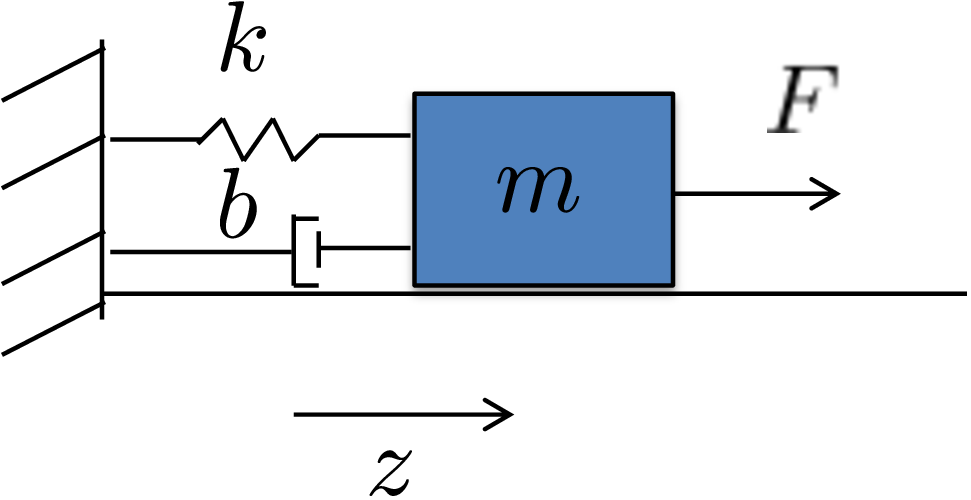
\includegraphics[width=0.4\textwidth]{6_design_studies/figures/hw_mass_defn}\\
  \caption{Mass Spring Damper}
  \label{fig:hw_mass_defn}
\end{figure}


